\question
\textbf{Trabalho Pr\'{a}tico 5 : Bobinas de Helmholtz}

Recorde o trabalho pr\'{a}tico sobre o estudo do campo magn\'{e}tico produzido pelas Bobinas de Helmholtz. Os resultados experimentais obtidos est\~{a}o representados no gr\'{a}fico da Fig.~\ref{fig:helmholtz}. Cada bobina tem de raio $R=3.5~\text{cm}$.

\begin{figure}[ht]
\centering
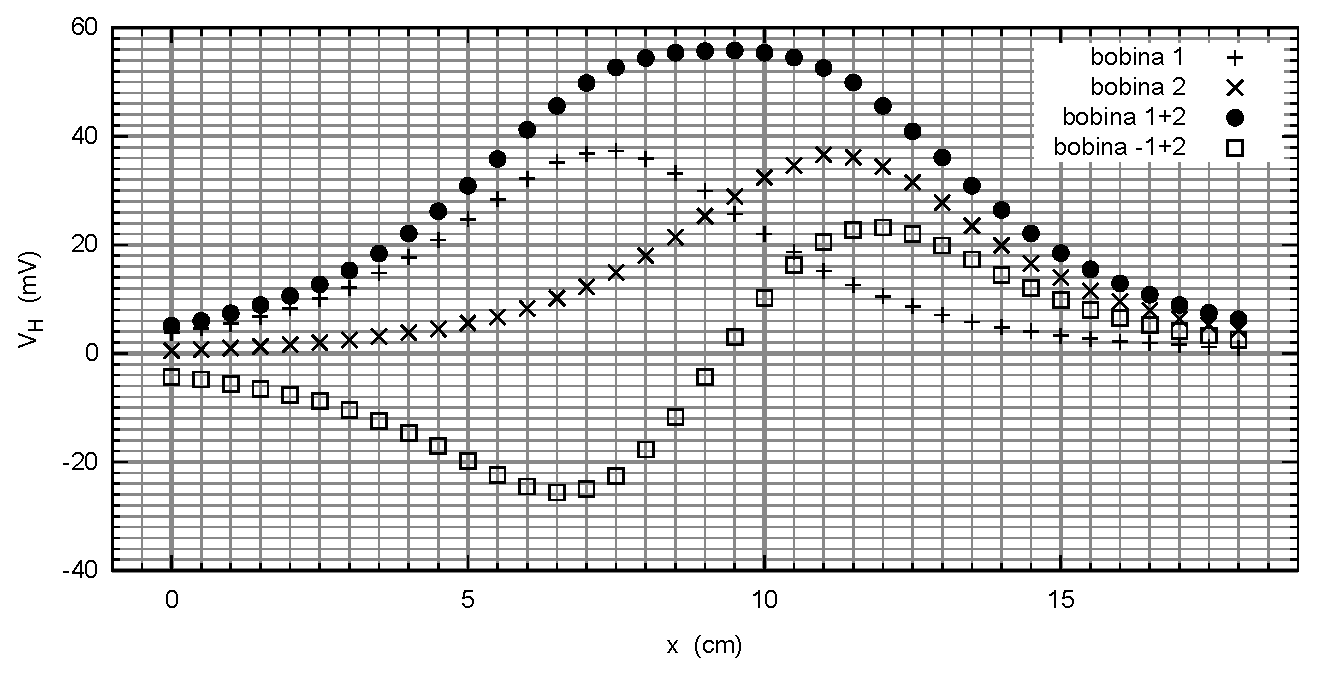
\includegraphics[scale=0.8]{gnuplot/helmholtz.eps}
\caption{\label{fig:helmholtz}Tens\~{a}o de Hall ao longo do eixo das bobinas.}
\end{figure}

\begin{parts}
\part[20]
A medi\c{c}\~{a}o do campo foi feita com recurso a uma sonda de efeito de Hall. Para a calibra\c{c}\~{a}o desta usou um solenoide padr\~{a}o. Diga em que posi\c{c}\~{a}o do solenoide colocou a sonda e porqu\^{e}.

\part[15]
Sabendo que a constante de calibra\c{c}\~{a}o da sonda $C_c \pm \Delta Cc = 34.9 \pm 0.5~\text{(mT/V)}$, determine o valor do campo magn\'{e}tico para a Bobina 2 e respetivo erro, na posi\c{c}\~{a}o $x=11.5~\text{cm}$.

\part[10]
Indique, justificando, se trabalhou em configura\c{c}\~{a}o de Helmholtz e indique tamb\'{e}m a principal vantagem desta configura\c{c}\~{a}o de bobinas.

\part[15]
Conclua, atrav\'{e}s do gr\'{a}fico, se se verifica ou n\~{a}o o princ\'{i}pio da sobreposi\c{c}\~{a}o do campo magnetico no caso em que as bobinas t\^{e}m corrente a fluir em sentidos opostos.

\part[15]
Determine o n\'{u}mero de espiras da bobina 2 se nesta estiver a fluir uma corrente de $I=0.585~\text{A}$, sabendo que o campo magn\'{e}tico por uma espira ao longo do seu eixo \'{e} dado pela Eq.~\ref{eq:coilfield}.

\begin{equation}
\label{eq:coilfield}
B\left(x\right)=\frac{\mu_0}{2}\frac{IR^2}{\left(R^2+x^2\right)^{3/2}}
\end{equation}
\end{parts}